\chapter{Czech datasets}
Czech language is a so-called "low resource language", which in the machine learning community means that, for particular languge, a limited number of datasets of sufficient quality  and size, is available. Thus, the bias detection task in Czech environment is complicated. Despite the relatively sufficient number of datasets in English, there is essentially no Czech one suitable.

 Essentially, three options to solve this problem are available. The most promising way is to annotate a new gold-standard dataset. However, media bias is a nontrivial, complex, and subtle linguistic feature , hence a lot of effort must be put into annotator training and eventual filtering of implicitly biased annotations.
 
 Another way is to use an automatic approach -> allsides.com , however, this leads to oversimplification and results in a very noisy dataset. Regardless, such dataset can still be used for domain-specific pretraining \cite{Spinde2021f}. Unfortunately, there is no Czech site that would provide useful bias information on neither source or article level. Server \Gls{nfnz} \footnote{https://www.nfnz.cz/} provides scoring for different news sources. Nonetheless, only a fraction of their scoring is related to the actual linguistic aspect of the source. Most of the scoring is based on meta-information such as transparency, proper citation, etc.
 
 Nonetheless, automatic creation of dataset can be done in a clever way like described in section \ref{wiki-npov}. Despite the limitation caused by the size of the particular Wikipedia, this approach is suitable for Czech environment, since Czech Wikipedia has a comparably large editor base \footnote{ \url{https://en.wikipedia.org/wiki/List_of_Wikipedias}} ranking 26. in a number of edits worldwide. I took this approach and I present a new parallel corpus for bias detection based on Czech Wikipedia \ref{wncs}.
 
 Finally, for low resource languages, it is reasonable to translate English datasets. As one of my main contributions in bias detection in Czech news, I translated most of the relevant datasets described in chapter \ref{datasets} using \textbf{DeepL}, and processed them into a unified format \ref{processing}. .
 
\section{Translation}

\textit{example of translated sentences}
\subsection{DeepL}
\section{Processing}\label{processing}
For convenience, every data point is in "sentence,label" format, where $label \in \{0,1\}$ stands for unbiased,biased, respectively. Thus, easy data merging and combination is possible.
\section{Analysis}
output = unified set of Czech bias related datasets\label{f}
\textbf{Czech Unified set of Bias Data}
\begin{enumerate}
    \item babe-cs
    \item basil-cs
    \item wikibias-cs
    \item cw-hard-cs
    \item mpqa-cs
    \item nfnj-cs
    \item subj-cs
    \item ua-crisis-cs
    \item wnc-cs
    \item wnc-large-cs ?
\end{enumerate}

\newpage

\section{Czech Wiki Neutrality Corpus}
Finally, I present two novel parallel corpora extracted directly from Czech Wikipedia. To my best knowledge, this is the only original Czech dataset related to media bias and subjectivity detection. The only related dataset is SubLex which is a subjectivity lexicon mainly focused on sentiment. However, lexicon based approaches proved to be insufficient in takcling complex media bias.

For the dataset creation, I followed two main existing approaches, both of them relying on the extraction of revisions that includes the \{\{NPOV\}\} tag or its variation. The NPOV tag has also its Czech version \Gls{nup}. However, the czech version is practically not used and so for the extraction, the english variations were used.

\subsubsection{WIKI1-CS}
For this dataset I followed the \cite{aleksandrova2019multilingual} approach and their script. First, a file with all pages and its complete edit history is downloaded from wiki dump. I used the "20220201" version. Then the edits containing one of the NPOV related tags are extracted and then the process of sentence extraction follows. All used tags can be seen in appendix.

This approach yielded 15k sentences, However, it uses rather trivial assumption that when NPOV tag is removed, all removed sentences are biased and all added are expected to be unbiased. This annotating strategy later [odkaz na experimenty] proved to be insuffiecient and yielded very noisy dataset. For this reason I excluded this dataset from further experiments.

\subsubsection{WIKI2-CS}\label{wncs}
This dataset was created following \cite{pryzant2020automatically} approach. The process is the same as described in section \ref{wiki}. I used "20220201" snapshot of wikipedia dump. I chose the latest version that included all the necessary files.
I used the script publicly available on github [odkaz na repo],with few slight modifications to fit the czech language properties:
\begin{enumerate}
    \item Regex was extended to exclude czech words that contain "pov" inside eg. povstání, povlak etc. \footnote{Regular expression used to match npov related comments: }
    \item All cases has been preserved, since bert like models can handle cased language.
    \item Czech Morphodita tokenizer was used.
\end{enumerate}
\newpage
Final dataset consists of:
\begin{enumerate}
    \item 3k of "before" and "after" sentence pairs
    \item 1.7k subset of mentioned set where only one word was changed
    \item 7.5 sentences, where the change was rejected or reversed implying neutrality of the original sentence
\end{enumerate}

The random example of sentence pair can be seen in \ref{fig:wiki2cs-example}

\begin{figure}
  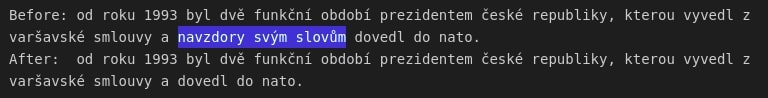
\includegraphics[width=\linewidth]{my_modules/multimedia/wiki2example.jpg}
  \caption{Example of CWNC sentence pair}
  \label{fig:wiki2cs-example}
\end{figure}

\section{Not translated}
Since my current DeepL plan allowed me to translate only one "large-scale" dataset due to the DeepL's fair usage policy I decided to not translate the NewsB since it focuses on distinguishing between conservative and liberal bias hence is not directly applicable on our task. However the hyperpartisan task is a good candidate for multi task setting as suggested later in \ref{mtl} section